% !TEX root = main.tex

\paragraph{Model} Let us consider a given Horn rule $\vec{B} \Rightarrow r(x,y)$. Let us look at all facts with relation $r$ (Figure \ref{model}). We distinguish 4 types of facts: True facts that are known to the KB (KBtrue), true facts that are unknown to the KB (NEWtrue), facts that are known to be false in the KB (KBfalse), and facts that are false but unknown to the KB (NEWfalse). The rule will make certain predictions (blue circle). These predictions can be known to be true (A), known to be false (C), or unknown (B and D). When they are unknown to the KB, they can still be true (B) or false (D) with respect to the real world.\\

\ffigure{Figure}{model}{Prediction under Incompleteness}{% This is the TIKZ version of the file
%     model.svg
% generated by PowerLine, the free SVG editor with Latex support

% To include this picture in LaTex, write the following in its preamble:
%  \usepackage{tikz}
%  \usepackage{graphicx}
%  \usepackage{hyperref}
% Then write '% !TEX root = main.tex

\www{
\paragraph{Model} We follow the description of the mining model from \cite{amie}.
Let us consider a given Horn rule $\vec{B} \Rightarrow r(x,y)$. Let us look at all facts with relation $r$ (Figure \ref{model}). 
We distinguish 4 types of facts: True facts that are known to the KB (KBtrue), true facts that are unknown to the KB (NEWtrue), 
facts that are known to be false in the KB (KBfalse), and facts that are false but unknown to the KB (NEWfalse). 
The rule will make certain predictions (blue circle). These predictions can be known to be true (A), known to be false (C), or unknown (B and D). 
When they are unknown to the KB, they can still be true (B) or false (D) with respect to the real world.\\

\ffigure{Figure}{model}{\label{fig:prediction}Prediction under Incompleteness}{% This is the TIKZ version of the file
%     model.svg
% generated by PowerLine, the free SVG editor with Latex support

% To include this picture in LaTex, write the following in its preamble:
%  \usepackage{tikz}
%  \usepackage{graphicx}
%  \usepackage{hyperref}
% Then write '\input{model.tikz}' where the picture shall appear in the LaTex document.

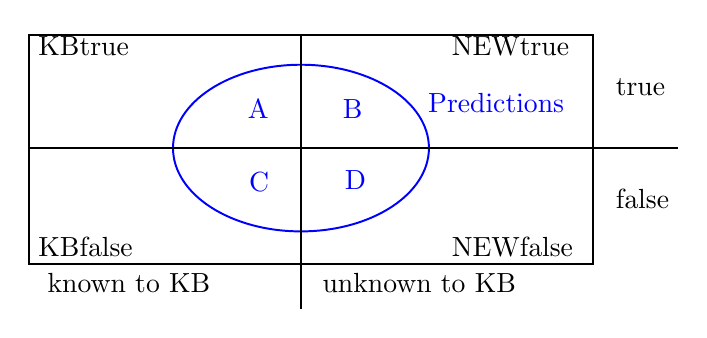
\begin{tikzpicture}

% Fabian: Keep figure in two colors.
% Even if printed in black and white, it's still clear enough

  \path[draw=blue, line width=0.7086614168764338] (3.708333, -1.458333) ellipse (1.625000 and 1.058333);
  \node[above, right, color=blue, font=] at (5.2000, -0.88333) {Predictions};
  \node[above, right, color=blue, font=] at (2.908333, -0.958333) {A};
  \node[above, right, color=blue, font=] at (4.116667, -0.966667) {B};
  \node[above, right, color=blue, font=] at (2.925000, -1.891667) {C};
  \node[above, right, color=blue, font=] at (4.141667, -1.866667) {D};
  \node[above, right, color=black, font=] at (0.250000, -0.166667) {KBtrue};
  \node[above, right, color=black, font=] at (0.250000, -2.708333) {KBfalse};
  \node[above, right, color=black, font=] at (5.500000, -0.166667) {NEWtrue};
  \node[above, right, color=black, font=] at (5.500000, -2.708333) {NEWfalse};
  \node[above, right, color=black, font=] at (7.583333, -0.683333) {true};
  \node[above, right, color=black, font=] at (7.583333, -2.100000) {false};
  \node[above, right, color=black, font=] at (0.366667, -3.166667) {known to KB};
  \node[above, right, color=black, font=] at (3.858333, -3.166667) {unknown to KB};
  \path[draw=black, line width=0.7086614168764338] (0.250000, -0.016667) rectangle (7.416667, -2.933333);
  \draw[draw=black, line width=0.7086614168764338] (0.250000, -1.458333) -- (8.500000, -1.458333);
  \draw[draw=black, line width=0.7086614168764338] (3.708333, -0.025000) -- (3.708333, -3.500000);
\end{tikzpicture}
}

}

\www{
\paragraph{Goal} 
Our goal is to find rules that make true predictions that go beyond the current KB. 
In the figure, we wish to maximize the area B, and to minimize the area D. 
There are two obvious challenges in this context: First, the areas NEWtrue and NEWfalse are unknown. 
So if we wish to maximize B at the expense of D, we are operating in an area outside our KB. 
We would want to use the areas KBtrue and KBfalse to estimate the unknown area. 
This, however, leads to the second challenge: Semantic KBs do not contain negative evidence. 
Thus, the area KBfalse is empty. In the following, we discuss different measures that address these challenges.
}

% \www{
% \paragraph{Support} 
% The \emph{support} of a rule quantifies the number of correct predictions, i.e., the size of A. There are several ways to define the support: It can be the number of instantiations of the rule that appear in the KB. This is what our analogy to association rule mining \cite{AgrImiSwa93} suggests (Section \ref{sec:preliminaries}). This measure, however, is not monotonic if we add atoms to the body. Consider, for example, the rule
% \indented{
%   \emph{marriedTo(}$x,y) \Rightarrow$ \emph{marriedTo(}$y,x$)
% }
% If we add \emph{hasGender($x$,male)} to the body, the number of instantiations that are in the KB decreases. If we add an atom with a fresh variable, e.g., \emph{hasFriend($x$,$z$)}, to the body, the number of instantiations increases for every friend of $x$. This is true even if we add another atom with $z$ to make the rule closed.\
% Alternatively, we can count the number of facts in one particular body atom.
% This definition, however, depends on the choice of the body atom, so that the same rule can have different supports. We can also count the number of facts of the head atom.
% This measure decreases monotonically if more body atoms are added 
% and avoids equivalent rules with different support values. With this in mind, we define the support of a rule as the number of distinct pairs of subjects and objects in the head of all instantiations that appear in the KB:
% \[supp(\vec{B} \Rightarrow r(x,y)) := \#(x,y): \exists z_1,...,z_m: \vec{B} \wedge r(x,y)\]
% where $z_1,...,z_m$ are the variables of the rule apart from $x$ and $y$.
% }

\www{
\paragraph{Support} 
The \emph{support} of a rule quantifies the number of correct predictions, i.e., the size of A. 
There are several ways to define the support: It can be the number of instantiations of the rule that appear in the KB. 
%This is what our analogy to association rule mining \cite{AgrImiSwa93} suggests (Section \ref{sec:preliminaries}). \comment{Katja}{Remove this sentence if the section about association rule mining is removed permanently.}
This measure, however, is not monotonic if we add atoms to the body. Consider, for example, the rule
\indented{
  \emph{marriedTo(}$x,y) \Rightarrow$ \emph{marriedTo(}$y,x$)
}
If we add \emph{hasGender($x$,male)} to the body, the number of instantiations that are in the KB decreases. 
If we add an atom with a fresh variable, e.g., \emph{hasFriend($x$,$z$)}, to the body, the number of instantiations increases for every friend of $x$. 
This is true even if we add another atom with $z$ to obtain a closed rule.\
Alternatively, we can count the number of facts in one particular body atom.
This definition, however, depends on the choice of the body atom, so that the same rule can have different supports. 
We can also count the number of facts of the head atom.
This measure decreases monotonically if more body atoms are added and avoids equivalent rules with different support values. 
With this in mind, we define the support of a rule as the number of distinct pairs of subjects and objects in the head of all instantiations that appear in the KB:
\[supp(\vec{B} \Rightarrow r(x,y)) := \#(x,y): \exists z_1,...,z_m: \vec{B} \wedge r(x,y)\]
where $z_1,...,z_m$ are the variables of the rule apart from $x$ and $y$. }
Note that the support is defined even for rules that are not closed.


% \www{
% \paragraph{Head Coverage} %\comment{check again}
% % Support is an absolute number. This means that a user who thresholds on support has to know the absolute size of the KB to give meaningful values. 
% % To avoid this, we also need to define a proportional version of support, the \emph{head coverage}. It is the proportion of pairs from the head relation that are covered by the predictions of the rule:
% % \[hc(\vec{B} \Rightarrow r(x,y)) := \frac{supp(\vec{B} \Rightarrow r(x,y))}{\#(x,y) : r(x,y)}\]
% Support is an absolute number. This means that a user who thresholds on support has to know the absolute size of the KB to give meaningful values. 
% To avoid this, we also define a proportional version of support. A naive way would be to use the absolute number of support, as defined in the previous paragraph, over the size of the KB. 
% In this case, however, relations that do not have many facts (either because of the incompleteness of the KB or because of their nature), will not be considered in the head of rules,
% i.e. we will not learn rules predicting such relations. Therefore, we propose to use the notion of \emph{head coverage}. 
% This is the proportion of pairs from the head relation that are covered by the predictions of the rule
% % Head coverage is the proportion of pairs from the head relation that are covered by the predictions of the rule:
% \[hc(\vec{B} \Rightarrow r(x,y)) := \frac{supp(\vec{B} \Rightarrow r(x,y))}{\#(x',y') : r(x',y')}\]
% }


\www{
\paragraph{Head Coverage}
Support is an absolute number. This means that a user defining thresholds on support has to know the absolute size of the KB to give meaningful values. 
To avoid this, we propose a proportional version of support. A naive way would be to use the absolute number of support, as defined in the previous paragraph, over the size of the KB. 
In this case, however, relations that do not have many facts (either because of the incompleteness of the KB or because of their nature) will not be considered in the head of the rules,
i.e., we will not learn rules predicting such relations. Therefore, we propose to use the notion of \emph{head coverage}:
\[hc(\vec{B} \Rightarrow r(x,y)) := \frac{supp(\vec{B} \Rightarrow r(x,y))}{size(r)}\]
}

with $size(r) := \#(x',y') : r(x',y')$ denoting the number of facts in relation $r$.

Head coverage quantifies the percentage of the known true facts that are implied %(for the case of closed rules) %or can possibly be implied (for the case of not yet closed rules)
% Fabian: I think that this description is sufficient. The mroe precise one risks confusing readers.
by the rule.
Head coverage can be a measure of statistical significance for any measure used to evaluate the quality of a rule. 
\comment{Fabian}{I am not sure about this. Could you explain? If it is not crucial here, I would omit it at this position.}



\www{
\paragraph{Negative Examples} 
The central challenge of our setting is to provide counter-examples for the rule mining. 
These can take the role of KBfalse, so that we can estimate the areas NEWtrue and NEWfalse. 
There are several approaches to this problem: The standard confidence, the standard positive-only learning evaluation score of ILP, and the partial completeness assumption that we propose. 
}
We will now present these approaches in detail.

% \www{
% \paragraph{Standard Confidence} 
% The standard confidence measure takes all facts that are not in the KB (i.e., NEWtrue and NEWfalse) as negative evidence. 
% Thus, the standard confidence of a rule is the ratio of its predictions that are in the KB, i.e., the share of A in the set of predictions:
% \[conf(\vec{B} \Rightarrow r(x,y)) := \frac{supp(\vec{B} \Rightarrow r(x,y))}{\#(x,y): \exists z_1,...,z_m: \vec{B}}\]
% %\[conf(\vec{B} \Rightarrow r(x,y)) := \frac{supp(\vec{B} \Rightarrow r(x,y))}{supp(\vec{B})}\]
% The standard confidence is blind to the distinction between ``false'' and ``unknown''. Thus, it implements a closed world setting. It mainly describes the known data and penalizes rules that make a large number of predictions in the unknown region. We, in contrast, aim to maximize the number of true predictions that go beyond the current knowledge. We do not want to describe data, but to predict data.
% }



\www{
\paragraph{Standard Confidence} 
The standard confidence measure takes all facts that are not in the KB (i.e., NEWtrue and NEWfalse) as negative evidence. 
Thus, the standard confidence of a rule is the ratio of its predictions that are in the KB, i.e., the share of A (KBtrue) in the set of predictions:
%\[conf(\vec{B} \Rightarrow r(x,y)) := \frac{supp(\vec{B} \Rightarrow r(x,y))}{\#(x,y): \exists z_1,...,z_m: \vec{B}}\]
}

%\comment{Katja}{I prefer the second one.}
\[conf(\vec{B} \Rightarrow r(x,y)) := \frac{\#(x,y): \exists z_1,...,z_m: \vec{B} \wedge r(x,y)}{\#(x,y): \exists z_1,...,z_m: \vec{B}}\]
%\[conf(\vec{B} \Rightarrow r(x,y)) := \frac{supp(\vec{B} \Rightarrow r(x,y))}{supp(\vec{B})}\]

Standard confidence is the measure traditionally used in association rule mining and market basket analysis, where a Closed World Assumption (CWA) is made: 
if there is no evidence in any of the transactions of the database that a user bought a specific product, then this user did not buy the product.
Although natural for the market basket analysis scenario, standard confidence fails to distinguish between ``false'' and ``unknown'' facts, 
which makes it inappropriate for a scenario with Open World semantics, like ours. Moreover, we also persue a different goal than market basket analysis:
we aim to maximize the number of true predictions that go beyond the current knowledge, whereas market basket analysis usually tries to mine rules that can describe data that is already known. 






\www{
\paragraph{Positive-Only Learning} 
For cases where the KB does not contain negative examples, Muggleton has developed a \emph{positive-only learning evaluation score} for ILP \cite{Muggleton:1996:LPD:647996.742465},\cite{usir1753}. 
It takes random facts as negative evidence:
\[
 Score = log(P)-log\frac{R+1}{Rsize+2}-\frac{L}{P}
\]
Here, $P$ is the number of known true facts covered (KBtree, or A resp., in Figure~\ref{fig:prediction}), $R$ is the number of randoms covered, $Rsize$ is the total number of randoms and $L$ is the number of atoms in the hypotheses. 
The intuition is that a good rule should cover many positive examples, and few or no randomly generated examples. This ensures  
that the rule is not overly general. Furthermore, the rule should use as few atoms as possible, and thus achieve a high compression. This measure is implemented (among others) in the ALEPH system.
}


% \www{
% \paragraph{Partial Completeness} 
% We propose to generate negative evidence by the \emph{partial completeness assumption} (PCA).
% This is the assumption that if $r(x,y) \in$ \emph{KBtrue} for some $x,y$, then
% \[\forall y': r(x,y') \in \mbox{\emph{KBtrue}} \cup \mbox{\emph{NEWtrue}} \Rightarrow r(x,y') \in \mbox{\emph{KBtrue}}\] 
% In other words, we assume that if the database knows some $r$-attribute of $x$, then it knows all $r$-attributes of $x$. This assumption is certainly true for functional relations $r$, 
% such as birth dates, capitals, etc. Thanks to the FUN-Property (see Section \ref{sec:model}), it is also true for inverse-functional relations, such as \emph{owns}, \emph{created}, etc. 
% The assumption is also true in the vast majority of cases for relations that are not functional, but that have a high functionality. 
% Even for other relations, the PCA is still reasonable for knowledge bases that have been extracted from a single source (such as DBpedia and YAGO). 
% These usually contain either all $r$-values or none for a given entity.
% }


\paragraph{Partial Completeness} 
We propose to generate negative evidence by means of the \emph{partial completeness assumption} (PCA).
This is the assumption that if $r(x,y) \in$ \emph{KBtrue} for some $x,y$,
%and $x$ is the input variable, 
% Fabian: we already said that all relations are more functional than inverse functional
then
\[\forall y': r(x,y') \in \mbox{\emph{KBtrue}} \cup \mbox{\emph{NEWtrue}} \Rightarrow r(x,y') \in \mbox{\emph{KBtrue}}\] 
%In other words, we assume that if the database knows some $r$-attribute of $x$, then it knows all $r$-attributes of $x$. 
%In other words, we assume that if the database knows some entity for the output variable $y$ for a given relation $r$ and entity of the input variable $x$, 
%then it knows all possible entities for the  output variable $y$ for these $r$ and $x$.
%\comment{Katja}{The term ``$r$-attribute of $x$'' is not intuitive for the reader as it has not been formally introduced, and the term attribute occurs only here. I suggest to replace it.}
% Fabian: I gave it another try, without the input and output:
In other words, we assume that if we know one $y$ for a given $x$, then we know all $y$ for that $x$.

This assumption is certainly true for functional relations $r$, such as \emph{birthdates} and \emph{capitals}.
Thanks to the FUN-property, the assumption is also true for inverse-functional relations, such as \emph{owns} and \emph{created}.
%, with the difference that in this case $x$ is the output variable and $y$ the input variable.
%, with the difference that in this case we assume that we know all $r$-attributes of $y$ (since $y$ is the input variable in this case).
The assumption is also true in the vast majority of cases for relations that are not functional, but that have a high functionality. 
Even for other relations, the PCA is still reasonable for knowledge bases that have been extracted from a single source (such as DBpedia and YAGO), as we shall see. 
%These usually contain either all $r$-values or none for a given entity. \comment{Katja}{Likewise, the term ``$r$-values'' is not introduced.}
We present an experimental evaluation of the PCA in Section~\ref{sec:experimentsPCA}.

% \www{
% \paragraph{PCA Confidence} 
% Under the PCA, we normalize the confidence not by the entire set of facts, but by the set of facts of which we know that they are true, together with the facts of which we assume that they are false. If the head atom of the rule is $r(x,y)$, then this set is just the set of facts $\{ r(x,y') : r(x,y') \in \mathcal{K}\}$. Thanks to the FUN-Property, the PCA is always applied to the first argument of the head atom:
% %\[pcaconf(\vec{B} \Rightarrow r(x,y)) := \frac{\#(x,y): \exists z_1,...,z_m: \vec{B} \wedge r(x,y)}{\#(x,y): \exists z_1,...,z_m,y': \vec{B} \wedge r(x,y')}\]
% \[pcaconf(\vec{B} \Rightarrow r(x,y)) := \frac{supp(\vec{B} \Rightarrow r(x,y))}{\#(x,y): \exists z_1,...,z_m,y': \vec{B} \wedge r(x,y')}\]
% We show in our experiments that the PCA confidence identifies much more productive rules than the other measures.
% }



\paragraph{PCA Confidence} 
\label{pcaConf}
Under the PCA, the denominator of the confidence will not be the size of the entire set of facts that the body of the rule produces, 
but the number of facts that we know to be true together with the facts that we assume to be false. 
\comment{Fabian}{Important fix here: Christina found that the denominator should count $\#(x,y)$, and not $\#(x,y')$.}

% If the head atom of the rule is $r(x,y)$, then this set is just the set of facts $\{ r(x,y') : r(x,y') \in \mathcal{K}\}$. 
% The PCA confidence for a rule with $x$ as the input variable is defined as:
% \[
% \small \hspace*{-1ex}
% conf_{PCA}(\vec{B} \Rightarrow r(x,y)) := \frac{supp(\vec{B} \Rightarrow r(x,y))}{\#(x,y): \exists z_1,...,z_m,y': \vec{B} \wedge r(x,y')}
% \]
% \comment{Katja}{If we replace the formula for the standard confidence, we should use the same notation here:
\[
\small \hspace*{-2ex}
conf_{PCA}(\vec{B} \Rightarrow r(x,y)) := \frac{\#(x,y): \exists z_1,...,z_m: \vec{B} \wedge r(x,y)}{\#(x,y): \exists z_1,...,z_m,y': \vec{B} \wedge r(x,y')}
\]
%}
This confidence normalizes the support by the number of pairs $(x,y)$ for which there exists a $y'$ with $r(x,y')$, i.e., for which we assume that the KB knows all such $y'$.
\comment{Chris}{Think about if you want to include the following one.} 
\comment{Katja}{I suggest to remove it because we will have a detailed discussion in the experiments and do not need it already here.}
The PCA confidence can be seen as a process in which we first take a biased sample of the body (those facts containing entities for the $x$ variable that appear also in the head)
and then calculate the standard confidence over this sample. 
The fact that our sample is biased implies that PCA confidence might not be a good estimator of the actual predictive power of the rule (precision).
However, our experiments show that overall PCA confidence identifies much more productive rules than the other measures and it also correlates with precision better than the standard confidence.' where the picture shall appear in the LaTex document.

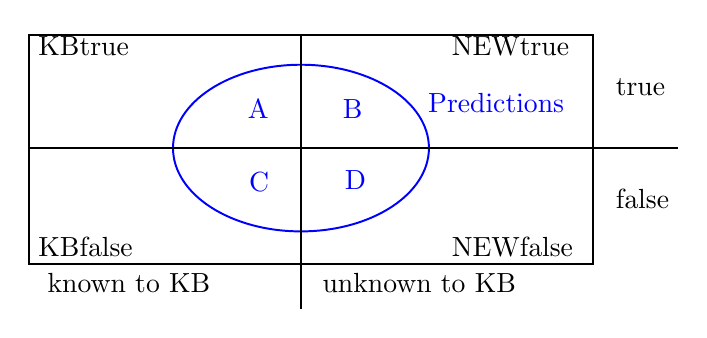
\begin{tikzpicture}

% Fabian: Keep figure in two colors.
% Even if printed in black and white, it's still clear enough

  \path[draw=blue, line width=0.7086614168764338] (3.708333, -1.458333) ellipse (1.625000 and 1.058333);
  \node[above, right, color=blue, font=] at (5.2000, -0.88333) {Predictions};
  \node[above, right, color=blue, font=] at (2.908333, -0.958333) {A};
  \node[above, right, color=blue, font=] at (4.116667, -0.966667) {B};
  \node[above, right, color=blue, font=] at (2.925000, -1.891667) {C};
  \node[above, right, color=blue, font=] at (4.141667, -1.866667) {D};
  \node[above, right, color=black, font=] at (0.250000, -0.166667) {KBtrue};
  \node[above, right, color=black, font=] at (0.250000, -2.708333) {KBfalse};
  \node[above, right, color=black, font=] at (5.500000, -0.166667) {NEWtrue};
  \node[above, right, color=black, font=] at (5.500000, -2.708333) {NEWfalse};
  \node[above, right, color=black, font=] at (7.583333, -0.683333) {true};
  \node[above, right, color=black, font=] at (7.583333, -2.100000) {false};
  \node[above, right, color=black, font=] at (0.366667, -3.166667) {known to KB};
  \node[above, right, color=black, font=] at (3.858333, -3.166667) {unknown to KB};
  \path[draw=black, line width=0.7086614168764338] (0.250000, -0.016667) rectangle (7.416667, -2.933333);
  \draw[draw=black, line width=0.7086614168764338] (0.250000, -1.458333) -- (8.500000, -1.458333);
  \draw[draw=black, line width=0.7086614168764338] (3.708333, -0.025000) -- (3.708333, -3.500000);
\end{tikzpicture}
}

\paragraph{Goal} Our goal is to find rules that make true predictions that go beyond the current KB. In the figure, we wish maximize the area B, and to minimize the area D. There are two obvious challenges in our context: First, the areas NEWtrue and NEWfalse are unknown. So if we wish to maximize B at the expense of D, we are operating in an area outside our KB. We would want to use the areas KBtrue and KBfalse to estimate the unknown area. This, however, leads to the second challenge: Semantic KBs do not contain negative evidence. Thus, the area KBfalse is empty. We will now present different measures that address these challenges.

\paragraph{Support} The \emph{support} of a rule quantifies the number of correct predictions, i.e., the size of A. There are several ways to define the support: It can be the number of instantiations of the rule that appear in the KB. This is what our analogy to association rule mining \cite{AgrImiSwa93} suggests (Section \ref{sec:preliminaries}). This measure, however, is not monotonic if we add atoms to the body. Consider, for example, the rule
\indented{
  \emph{marriedTo(}$x,y) \Rightarrow$ \emph{marriedTo(}$y,x$)
}
If we add \emph{hasGender($x$,male)} to the body, the number of instantiations that are in the KB decreases. If we add an atom with a fresh variable, e.g., \emph{hasFriend($x$,$z$)}, to the body, the number of instantiations increases for every friend of $x$. This is true even if we add another atom with $z$ to make the rule closed.\
Alternatively, we can count the number of facts in one particular body atom.
This definition, however, depends on the choice of the body atom, so that the same rule can have different supports. We can also count the number of facts of the head atom.
This measure decreases monotonically if more body atoms are added 
and avoids equivalent rules with different support values. With this in mind, we define the support of a rule as the number of distinct pairs of subjects and objects in the head of all instantiations that appear in the KB:
\[supp(\vec{B} \Rightarrow r(x,y)) := \#(x,y): \exists z_1,...,z_m: \vec{B} \wedge r(x,y)\]
where $z_1,...,z_m$ are the variables of the rule apart from $x$ and $y$.

\paragraph{Head Coverage} %\comment{check again}
% Support is an absolute number. This means that a user who thresholds on support has to know the absolute size of the KB to give meaningful values. 
% To avoid this, we also need to define a proportional version of support, the \emph{head coverage}. It is the proportion of pairs from the head relation that are covered by the predictions of the rule:
% \[hc(\vec{B} \Rightarrow r(x,y)) := \frac{supp(\vec{B} \Rightarrow r(x,y))}{\#(x,y) : r(x,y)}\]
Support is an absolute number. This means that a user who thresholds on support has to know the absolute size of the KB to give meaningful values. 
To avoid this, we also define a proportional version of support. A naive way would be to use the absolute number of support, as defined in the previous paragraph, over the size of the KB. 
In this case, however, relations that do not have many facts (either because of the incompleteness of the KB or because of their nature), will not be considered in the head of rules,
i.e. we will not learn rules predicting such relations. Therefore, we propose to use the notion of \emph{head coverage}. 
This is the proportion of pairs from the head relation that are covered by the predictions of the rule
% Head coverage is the proportion of pairs from the head relation that are covered by the predictions of the rule:
\[hc(\vec{B} \Rightarrow r(x,y)) := \frac{supp(\vec{B} \Rightarrow r(x,y))}{\#(x',y') : r(x',y')}\]

\paragraph{Negative Examples} The central challenge of our setting is to provide counter-examples for the rule mining. These can take the role of KBfalse, so that we can estimate the areas NEWtrue and NEWfalse. There are several approaches to this problem: The standard confidence, the standard positive-only learning evaluation score of ILP, and our new partial completeness assumption.

\paragraph{Standard Confidence} The standard confidence measure takes all facts that are not in the KB (i.e., NEWtrue and NEWfalse) as negative evidence. Thus, the standard confidence of a rule is the ratio of its predictions that are in the KB, i.e., the share of A in the set of predictions:
\[conf(\vec{B} \Rightarrow r(x,y)) := \frac{supp(\vec{B} \Rightarrow r(x,y))}{\#(x,y): \exists z_1,...,z_m: \vec{B}}\]
%\[conf(\vec{B} \Rightarrow r(x,y)) := \frac{supp(\vec{B} \Rightarrow r(x,y))}{supp(\vec{B})}\]
The standard confidence is blind to the distinction between ``false'' and ``unknown''. Thus, it implements a closed world setting. It mainly describes the known data and penalizes rules that make a large number of predictions in the unknown region. We, in contrast, aim to maximize the number of true predictions that go beyond the current knowledge. We do not want to describe data, but to predict data.

\paragraph{Positive-Only Learning} For cases where the KB does not contain negative examples, Muggleton has developed a \emph{positive-only learning evaluation score} for ILP \cite{Muggleton:1996:LPD:647996.742465},\cite{usir1753}. 
It takes random facts as negative evidence:
\[
 Score = log(P)-log\frac{R+1}{Rsize+2}-\frac{L}{P}
\]
Here, $P$ is the number of known true facts covered (A in the figure), $R$ is the number of randoms covered, $Rsize$ is the total number of randoms and $L$ is the number of atoms in the hypothesis. 
The intuition is that a good rule should cover many positive examples, and few or no randomly generated examples. This ensures  
that the rule is not overly general. Furthermore, the rule should use as few atoms as possible, and thus achieve a high compression. This measure is implemented (among others) in the ALEPH system.

\paragraph{Partial Completeness} We propose to generate negative evidence by the \emph{partial completeness assumption} (PCA).
This is the assumption that if $r(x,y) \in$ \emph{KBtrue} for some $x,y$, then
\[\forall y': r(x,y') \in \mbox{\emph{KBtrue}} \cup \mbox{\emph{NEWtrue}} \Rightarrow r(x,y') \in \mbox{\emph{KBtrue}}\] 
In other words, we assume that if the database knows some $r$-attribute of $x$, then it knows all $r$-attributes of $x$. This assumption is certainly true for functional relations $r$, 
such as birth dates, capitals, etc. Thanks to the FUN-Property (see Section \ref{sec:model}), it is also true for inverse-functional relations, such as \emph{owns}, \emph{created}, etc. 
The assumption is also true in the vast majority of cases for relations that are not functional, but that have a high functionality. 
Even for other relations, the PCA is still reasonable for knowledge bases that have been extracted from a single source (such as DBpedia and YAGO). 
These usually contain either all $r$-values or none for a given entity.

\paragraph{PCA Confidence} Under the PCA, we normalize the confidence not by the entire set of facts, but by the set of facts of which we know that they are true, together with the facts of which we assume that they are false. If the head atom of the rule is $r(x,y)$, then this set is just the set of facts $\{ r(x,y') : r(x,y') \in \mathcal{K}\}$. Thanks to the FUN-Property, the PCA is always applied to the first argument of the head atom:
%\[pcaconf(\vec{B} \Rightarrow r(x,y)) := \frac{\#(x,y): \exists z_1,...,z_m: \vec{B} \wedge r(x,y)}{\#(x,y): \exists z_1,...,z_m,y': \vec{B} \wedge r(x,y')}\]
\[pcaconf(\vec{B} \Rightarrow r(x,y)) := \frac{supp(\vec{B} \Rightarrow r(x,y))}{\#(x,y): \exists z_1,...,z_m,y': \vec{B} \wedge r(x,y')}\]
We show in our experiments that the PCA confidence identifies much more productive rules than the other measures.

\ignore{
\comment{Fabian}{The following might just go away}

\paragraph{Predictiveness} There is a third measure that we wish to maximize. We wish to make our rule predict true facts that are not yet in the database, i.e., we wish to maximize B. Unfortunately, B is unknown, so that we cannot estimate it. However, we can estimate $B \cup D$. 
We define the predictiveness of a rule as the ratio of unknown predictions out of the total number of predictions:
\[pred(\vec{B} \Rightarrow r(x,y)) := 1-\frac{\#(x,y): \exists z_1,...,z_m,y: \vec{B} \wedge r(x,y')}{\#(x,y): \exists z_1,...,z_m,y: \vec{B}}\]
%if $fun(r) \geq ifun(r)$. If the relation is more inverse functional, the formula is symmetric.
The higher the predictiveness, the more facts the rule will produce.

\paragraph{Size} The \emph{size} of a rule quantifies the total number of predictions, i.e., the size of $A \cup B \cup C \cup D$. This is just the number of head subjects for which the body holds:
\[size(\vec{B} \Rightarrow r(x,y)) := \#x: \exists z_1,...,z_m,x,y: \vec{B}\]
If we assume that the ratio of correct predictions is the same among the known facts and among the unknown facts, we can estimate the size of B as:
\[size(\vec{B} \Rightarrow r(x,y)) \times pcaconf(\vec{B} \Rightarrow r(x,y)) \times pred(\vec{B} \Rightarrow r(x,y))\]


Classical association rule mining and classical ILP are concerned with maximizing the number of true predictions of the rules, while minimizing the number of the false predictions of the rules. Here, ``true'' and ``false'' are to be understood with respect to the KB. That is, the classical approaches aim to maximize A, and minimize C. Thus, these approaches mainly describe the known data. They are blind to the predictions of the rule that go beyond the examples and counter examples: The realm of B and D. We, in contrast, aim to maximize the number of true predictions that go beyond the current knowledge. We do not want to describe 
but predict data. That is, we want to maximize B, the number of correct but yet unknown predictions. This is a very different setting, which requires the introduction of new metrics to estimate B and D.
}